\section{Reversible implementation}
As mentioned in section \ref{sec:fourier},
both FT and DFT are invertible sums.
The definition of IDFT also permits a factorization that is essentially equivalent to that of DFT.
However, we wish to write a reversible DFT that can be directly inverted to obtain an IDFT.
There are some challenges that must be overcome in order to do this.
The primary challenges are detailed in \cite{intfft},
which presents some solutions to these.

\subsection{Fixpoint arithmetic}
The first problem is that we must find a way to represent complex numbers.
Complex numbers are generally represented by $a, b \in \mathbb{R}$ such that $n = a + bi$.
You might normally choose to use floating point numbers to represent $a$ and $b$,
but updates to these are inherently destructive once.

Instead, we use a fix-point representation.
We represent real numbers by $r = x \cdot 2^{-p},~~ x, p \in \mathbb{Z}$.
The value of $p$ is known as the fix-point for $r$.
We will store $r$ in an integer, and $p$ will be implicit for the most part.
Operations on these numbers can be performed with the integer equivalents on the $x$ value.

Ignoring overflows, both addition and subtraction are invertible.
Multiplication is only injective ie. left-invertible.
This is quite clear when you consider what happens when dividing an odd number by 2.
Furthermore, it should be noted that multiplication of two numbers with fix-points $p_1$ and $p_2$
results in a number with fix-point $p_1 + p_2$.
When not updating in-place,
we can round off the lower bits of multiplication-results to keep the fix-point in place.

\subsection{Lifting steps}
\begin{figure}
    \centering
    \begin{subfigure}[b]{0.45\textwidth}
        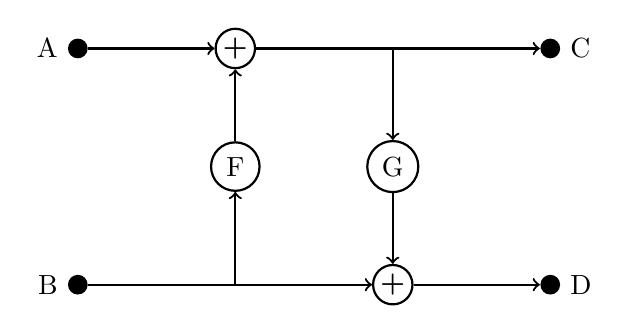
\begin{tikzpicture}[
                dot/.style = {circle, fill, inner sep = 0mm, minimum size = 2.5mm},
                op/.style = {draw, thick, circle, inner sep = 0mm, minimum size = 5mm},
                func/.style = {draw, thick, circle, inner sep = 1mm},
                arr/.style = {draw, thick, ->},
            ]
            \node (A) at (0, 3) [dot, label = left:A] {};
            \node (B) at (0, 0) [dot, label = left:B] {};
            \node (C) at (6, 3) [dot, label = right:C] {};
            \node (D) at (6, 0) [dot, label = right:D] {};

            \node (P1) at (2, 3) [op] {\textbf{+}};
            \node (P2) at (4, 0) [op] {\textbf{+}};

            \node (F) at (2, 1.5) [func] {F};
            \node (G) at (4, 1.5) [func] {G};

            \path[arr] (A) -- (P1);
            \path[arr] (P1) -- (C);
            \path[arr] (B) -- (P2);
            \path[arr] (P2) -- (D);
            \path[arr] (2, 0) -- (F);
            \path[arr] (F) -- (P1);
            \path[arr] (4, 3) -- (G);
            \path[arr] (G) -- (P2);
        \end{tikzpicture}
        \caption{Lifting steps.}
    \end{subfigure}
    \begin{subfigure}[b]{0.5\textwidth}
        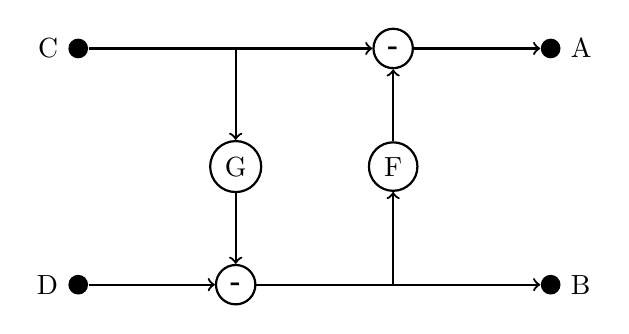
\begin{tikzpicture}[
                dot/.style = {circle, fill, inner sep = 0mm, minimum size = 2.5mm},
                op/.style = {draw, thick, circle, inner sep = 0mm, minimum size = 5mm},
                func/.style = {draw, thick, circle, inner sep = 1mm},
                arr/.style = {draw, thick, ->},
            ]
            \node (A) at (14, 3) [dot, label = right:A] {};
            \node (B) at (14, 0) [dot, label = right:B] {};
            \node (C) at (8, 3) [dot, label = left:C] {};
            \node (D) at (8, 0) [dot, label = left:D] {};

            \node (P1) at (12, 3) [op] {\textbf{-}};
            \node (P2) at (10, 0) [op] {\textbf{-}};

            \node (F) at (12, 1.5) [func] {F};
            \node (G) at (10, 1.5) [func] {G};

            \path[arr] (P1) -- (A);
            \path[arr] (C) -- (P1);
            \path[arr] (P2) -- (B);
            \path[arr] (D) -- (P2);

            \path[arr] (12, 0) -- (F);
            \path[arr] (10, 3) -- (G);
            \path[arr] (F) -- (P1);
            \path[arr] (G) -- (P2);
        \end{tikzpicture}
        \caption{Inverse path.}
    \end{subfigure}
    \caption{Dataflow path of a lifting step and its derived inverse.\label{fig:lift}}
\end{figure}

\subsection{Complex multiplication}
\begin{figure}
    \begin{subfigure}[b]{0.5\textwidth}
        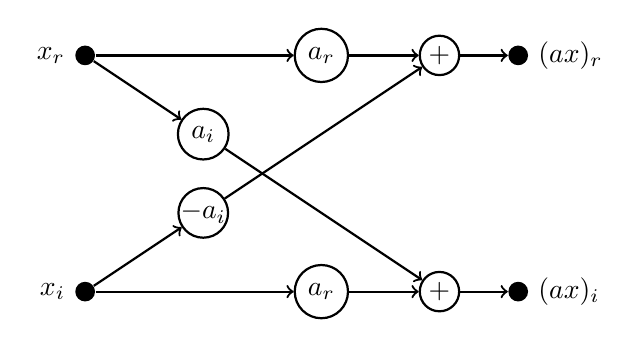
\begin{tikzpicture}[
                dot/.style = {circle, fill, inner sep = 0mm, minimum size = 2.5mm},
                op/.style = {draw, thick, circle, inner sep = 0mm, minimum size = 5mm},
                func/.style = {draw, thick, circle, inner sep = 1mm},
                arr/.style = {draw, thick, ->},
            ]
            \node (XR) [dot, label=left:$x_r$] at (0,3){};
            \node (XI) [dot, label=left:$x_i$] at (0,0){};
            \node (AXR) [dot, label=right:$(ax)_r$] at (5.5,3){};
            \node (AXI) [dot, label=right:$(ax)_i$] at (5.5,0){};

            \node (P1) [op] at (4.5, 3) {+};
            \node (P2) [op] at (4.5, 0) {+};
            \node (AR1) [func] at (3.0, 3) {$a_r$};
            \node (AR2) [func] at (3.0, 0) {$a_r$};

            \node (AI1) [func] at (1.5, 2) {$a_i$};
            \node (AI2) [op] at (1.5, 1) {$-a_i$};

            \path[arr] (XR) -- (AR1);
            \path[arr] (AR1) -- (P1);
            \path[arr] (P1) -- (AXR);

            \path[arr] (XI) -- (AR2);
            \path[arr] (AR2) -- (P2);
            \path[arr] (P2) -- (AXI);

            \path[arr] (XR) -- (AI1);
            \path[arr] (AI1) -- (P2);

            \path[arr] (XI) -- (AI2);
            \path[arr] (AI2) -- (P1);
        \end{tikzpicture}
        \caption{Butterfly structure.\label{fig:complexmula}}
    \end{subfigure}
    \begin{subfigure}[b]{0.5\textwidth}
        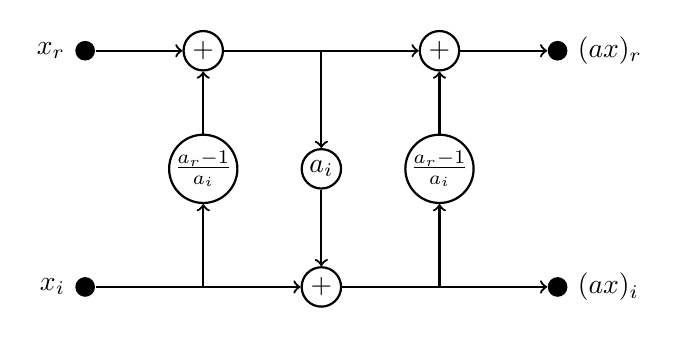
\begin{tikzpicture}[
                dot/.style = {circle, fill, inner sep = 0mm, minimum size = 2.5mm},
                op/.style = {draw, thick, circle, inner sep = 0mm, minimum size = 5mm},
                func/.style = {draw, thick, circle, inner sep = 1mm},
                arr/.style = {draw, thick, ->},
            ]
            \node (xr) [dot, label=left:$x_r$] at (0,3){};
            \node (xi) [dot, label=left:$x_i$] at (0,0){};
            \node (axr) [dot, label=right:$(ax)_r$] at (6,3){};
            \node (axi) [dot, label=right:$(ax)_i$] at (6,0){};

            \node (one) [op] at (1.5, 1.5) {$\frac{a_r - 1}{a_i}$};
            \node (two) [op] at (3, 1.5) {$a_i$};
            \node (three) [op] at (4.5, 1.5) {$\frac{a_r - 1}{a_i}$};

            \node (p1) [op] at (1.5, 3){+};
            \node (p2) [op] at (3, 0){+};
            \node (p3) [op] at (4.5, 3){+};

            \path[arr] (xr) -- (p1);
            \path[arr] (p1) -- (p3);
            \path[arr] (p3) -- (axr);

            \path[arr] (xi) -- (p2);
            \path[arr] (p2) -- (axi);

            \path[arr] (1.5, 0) -- (one);
            \path[arr] (one) -- (p1);

            \path[arr] (3, 3) -- (two);
            \path[arr] (two) -- (p2);

            \path[arr] (4.5, 0) -- (three);
            \path[arr] (three) -- (p3);
        \end{tikzpicture}
        \caption{Alternative lifting steps.\label{fig:complexmulb}}
    \end{subfigure}
    \caption{Datapaths for complex multiplication.\label{fig:complexmul}}
\end{figure}

\subsection{Reversible convolution}
\begin{figure}
    \centering
    \begin{subfigure}[b]{0.496\textwidth}
        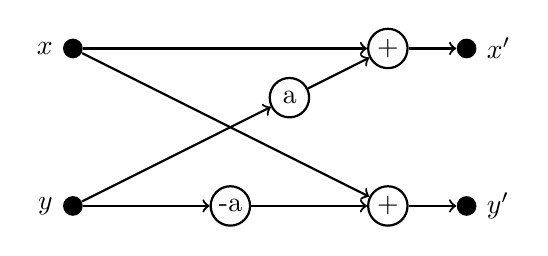
\begin{tikzpicture}[
                dot/.style = {circle, fill, inner sep = 0mm, minimum size = 2.5mm},
                op/.style = {draw, thick, circle, inner sep = 0mm, minimum size = 5mm},
                func/.style = {draw, thick, circle, inner sep = 1mm},
                arr/.style = {draw, thick, ->},
            ]
            \node (x) [dot, label=left:$x$] at (0,2){};
            \node (y) [dot, label=left:$y$] at (0,0){};
            \node (xp) [dot, label=right:$x'$] at (5,2){};
            \node (yp) [dot, label=right:$y'$] at (5,0){};

            \node (a1) [op] at (2.75, 1.375) {a};
            \node (a2) [op] at (2, 0) {-a};
            \node (p1) [op] at (4, 2) {+};
            \node (p2) [op] at (4, 0) {+};

            \path[arr] (x) -- (p1);
            \path[arr] (p1) -- (xp);
            \path[arr] (y) -- (a2);
            \path[arr] (a2) -- (p2);
            \path[arr] (p2) -- (yp);

            \path[arr] (x) -- (p2);

            \path[arr] (y) -- (a1);
            \path[arr] (a1) -- (p1);
        \end{tikzpicture}
        \caption{Butterfly structure.\label{fig:conva}}
    \end{subfigure}
    \begin{subfigure}[b]{0.496\textwidth}
        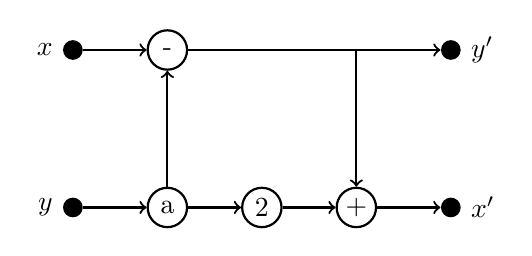
\begin{tikzpicture}[
                dot/.style = {circle, fill, inner sep = 0mm, minimum size = 2.5mm},
                op/.style = {draw, thick, circle, inner sep = 0mm, minimum size = 5mm},
                func/.style = {draw, thick, circle, inner sep = 1mm},
                arr/.style = {draw, thick, ->},
            ]
            \node (x) [dot, label=left:$x$] at (0,2){};
            \node (y) [dot, label=left:$y$] at (0,0){};
            \node (yp) [dot, label=right:$y'$] at (4.8,2){};
            \node (xp) [dot, label=right:$x'$] at (4.8,0){};

            \node (a) [op] at (1.2,0){a};
            \node (t) [op] at (2.4,0){2};
            \node (m) [op] at (1.2,2){-};
            \node (p) [op] at (3.6,0){+};

            \path[arr] (x) -- (m);
            \path[arr] (m) -- (yp);
            \path[arr] (y) -- (a);
            \path[arr] (a) -- (m);
            \path[arr] (a) -- (t);
            \path[arr] (t) -- (p);
            \path[arr] (p) -- (xp);
            \path[arr] (3.6,2) -- (p);
        \end{tikzpicture}
        \caption{Alternative lifting steps.\label{fig:convb}}
    \end{subfigure}
    \caption{Datapaths for FFT convolution.\label{fig:conv}}
\end{figure}

\begin{lstlisting}
procedure mul2
    if y = 0 then
        y += x
        x += y
        y -= x / 2
    fi y = 0
\end{lstlisting}

% TODO: Mention that the paper doesn't actually try to make directly reversible convolution

\begin{lstlisting}
x -= y
call mul2
y += x
x <=> y
\end{lstlisting}
